\documentclass{article}
\usepackage[utf8]{inputenc}
\usepackage[english, russian] {babel}
\usepackage{amsmath, amsfonts, amssymb}

\usepackage{graphicx}
\usepackage{float}
\usepackage{wrapfig}

\usepackage{xcolor}
\usepackage{hyperref}
\definecolor{linkcolor}{HTML}{799B03} 
\definecolor{urlcolor}{HTML}{799B03} 
\hypersetup{pdfstartview=FitH,  linkcolor=linkcolor,urlcolor=urlcolor, colorlinks=true}

\usepackage[answerdelayed, lastexercise]{exercise}

\usepackage{braket}

\documentclass{standalone}
\usepackage{tikzlings}
\usepackage{tikzducks}

\begin{document}
\begin{center}
\textbf{\huge{Гайд по школьной теории графов}}
\end{center}

\begin{flushleft}
\textbf{\Large{\begin{itemize}
\item Определения и факты
\item Деревья
\item Пути, циклы, связность
\item Теорема Турана
\item Двудольные графы
\item Задачи с олимпиад последних лет
\item Ссылки
\end{itemize}}}

\footnotetext{
\url{https://github.com/Aksinya-Bykova/olympiad-math} обновление версий гайда и задачи по графам с олимпиад без гайда -- посмотрите актуальную версию, пожалуйста
\newline
Telegram \url{https://t.me/Aksinya_By}
}
\end{flushleft}
\pagestyle{empty}

\newpage
\pagestyle{plain}
\normalsize

\begin{figure}[h!]
\centering
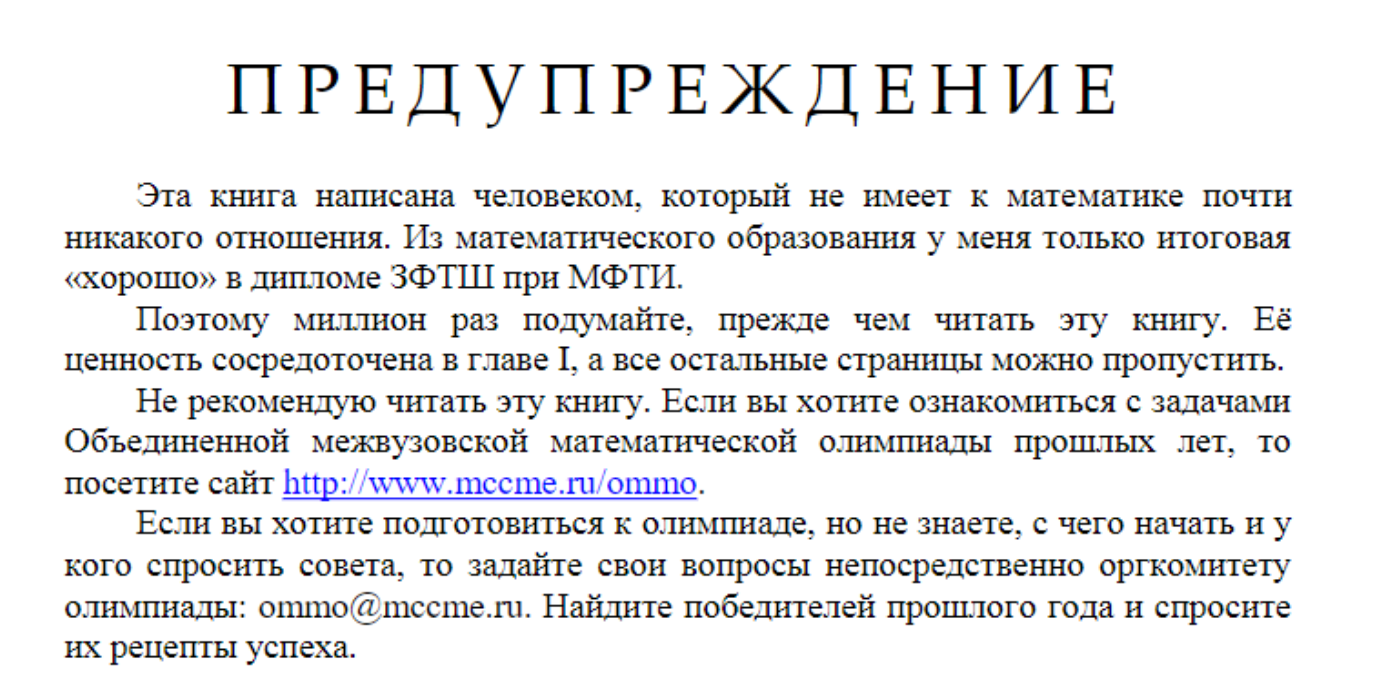
\includegraphics[width=0.8\linewidth]{warning.png}
\label{fig:mpr}
\caption{Немного об ОММО, изд. 2019}
\end{figure}

Я создавала эту книгу с идеей помочь тем, кто, как и я в своё время, оказался наедине с олимпиадной подготовкой, без сильного кружка или с сильным кружком, но в позиции отстающего. 
\\
\\
Так уж вышло, что под руку мне попалась теория графов -- у меня был школьный проект по этой теме. И на тот момент в интернете не существовало хороших гайдов по изучению или хотя бы подборок, иногда мне встречались листочки каких-то кружков. 
\\
\\
Я ни разу не великий графолог, в этой точке жизни даже не математик, а скорее инженер. Моя программа в ИТМО называется Software engineering. Так что надеюсь на ваше критическое мышление.

\newpage
\section{Определения и факты}

\subsection{Базовая теория}
\begin{itemize}
\item \href{https://clck.ru/DRCAR}{Основные определения теории графов}
\item \href{https://mathus.ru/math/graphs-tree.pdf}{Дерево, эквивалентные определения, доказательство их равносильности}
\item \href{http://neerc.ifmo.ru/wiki/index.php?title=%D0%9B%D0%B5%D0%BC%D0%BC%D0%B0_%D0%BE_%D1%80%D1%83%D0%BA%D0%BE%D0%BF%D0%BE%D0%B6%D0%B0%D1%82%D0%B8%D1%8F%D1%85}{Лемма о рукопожатиях}(\href{http://mmmf.msu.ru/archive/20132014/z6/12.04.2014.html}{задачи})
\item \href{https://mathus.ru/math/fepg.pdf}{Формула Эйлера в планарных графах}
\item \href{https://www.mccme.ru/s43/math/uroki/2009_2010/9mat_0910/spec/59_hall_lect.pdf}{Лемма Холла}
\item \href{https://neerc.ifmo.ru/wiki/index.php?title=%D0%A2%D1%83%D1%80%D0%BD%D0%B8%D1%80%D1%8B}{Турниры}
\item Задача Рамсея
\item \href{https://mathus.ru/math/teorema-turana.pdf}{Теорема Турана}
\end{itemize}

\subsection{Для интересующихся (например, следующее)}
\begin{itemize}
\item Формула Эйлера и многогранники
\item Гамильтонов путь в полных орграфах
\item \href{https://math.mosolymp.ru/upload/files/2022/khamovniki/8/8-2/8-2__Seriya_13__Ei%CC%86lerovyi_grafyi_i_lemma_o_horovodah.pdf}{Критерий эйлерова графа, лемма о хороводах}
\item \href{https://math.mosolymp.ru/upload/files/2018/other/444/10-11/2017_09_19_444_10-11_kyonig_diluors.pdf}{Теоремы Кёнига, Дилуорса}
\item \href{https://math.mosolymp.ru/upload/files/2022/khamovniki/11/11-1/2021-10-28_Teorema_Forda-Falkersona.pdf}{Теоремы Менгера, Форда-Фалкерсона}
\item Теоремы Дирака, Оре
\item Теорема Мирского
\item Теорема Ван дер Вардена
\end{itemize}
\\
\\
Я постаралась оставить в базовой части только действительно необходимое, и даже опросила своих друзей и знакомых для этого.


\newpage
\section{Рандом задачи}
\begin{itemize}
\subsection{Часть 1}
\item Сформулировать лемму о рукопожатиях.
\item Сколько рёбер в полном графе на n вершинах?
\item Способы задания графа.
\item Строго докажите, что в дереве на n вершинах ровно n - 1 рёбер.
\item Что значит "связный, без кратных рёбер и петель"? Зачем это уточнять?
\item Что такое простой граф? 
\item Опровергните популярное в интернете утверждение о том, что уровень твоего богатства/интеллекта -- среднее арифметическое уровня твоих 5 самых близких людей.
\newline
Есть два смешных видео по этому поводу: \url{https://www.youtube.com/watch?v=iwZE4OQ7HQU} -- убеждение в этом (без негатива, вряд ли это было со зла), \url{https://www.youtube.com/watch?v=FhCE54wLNZA} -- интуитивное опровержение, без строгого доказательства, зато с визуализацией.
\item Каким способом можно обойти все вершины связного графа? Приведите любой алгоритм. 
\item Расширенная задача Рамсея. Рёбра полного графа на 6 вершинах покрашены в синий и красный. Докажите, что в нём найдётся два одноцветных треугольника.
\end{itemize}

\subsection{Часть 2}
\begin{itemize}
\item Что такое планарный граф? Приведите пример не планарного графа. 
\item Что такое биекция (отношение) и каково её графическое представление? Приведите пример задачи, когда рёбра означают соответствие или отсутствие соответствия, а не дороги/знакомства между людьми.
\item Какова высота двоичного дерева, если оно состоит из вершины и двух поддеревьев с ней связанных, причём отличающихся по высоте не более чем на 1? (см. AVL-дерево \url{https://www.youtube.com/watch?v=Iee0SUyi35E})
\item Приведите хотя бы один пример применения дерева.
\item Что такое "антиграф" или дополнительный граф?
\item Что такое клика?
\item Докажите, что правильных многогранников в 3D -- 5.
\item Что такое эйлеров и гамильтонов графы?
\item В связном графе степень каждой вершины чётная. Докажите, что в нём существует эйлеров цикл.
\item Докажите, что в полном ориентированном графе есть гамильтонов путь.
\item Что означает умножание матриц? Почему оно не коммутативно? Зачем перемножать матрицу смежности связного графа с собой несколько раз?
\item Сформулируйте теорему Турана и докажите.
\end{itemize}

\newpage
\section{Ответы }
\subsection{Часть 1}

\begin{itemize}
\item \textbf{Сформулировать лемму о рукопожатиях.}
\newline
Сумма степеней вершин равна удвоенному числу рёбер.
\item \textbf{Сколько рёбер в полном графе на n вершинах?}
\newline
$\frac{n(n - 1)}{2}$
\item \textbf{Способы задания графа.}
\newline
Графически (палочки и кружочки), матрица смежности, список смежности. Это самые популярные.
\item \textbf{Строго докажите, что в дереве на n вершинах ровно n - 1 рёбер.}
\newline
Заметим, что любой подграф дерева -- по определению дерево. Утверждение можно доказать по индукции.
\item \textbf{Что значит "связный, без кратных рёбер и петель"? Зачем это уточнять?}
\newline
Связный -- между любыми двумя вершинами существует путь. Кратные рёбра -- несколько рёбер между двумя вершинами. Петля -- ребро из вершины в ту же вершину. Намёк: когда вы говорите "граф", неочевидно, что он именно такой.
\item \textbf{Что такое простой граф?} 
\newline
Граф без кратных рёбер и петель (необязательно связный).
\item \textbf{Опровергните популярное в интернете утверждение о том, что уровень твоего богатства/интеллекта -- среднее арифметическое уровня твоих 5 самых близких людей.}
\newline
Рассмотрим самого богатого человека, тогда его друзья тоже самые богатые. Значит, все люди самые богатые, если граф людей считать связным. Это неправда. 
\item \textbf{Каким способом можно обойти все вершины связного графа? Приведите любой алгоритм.}
\newline
DFS, BFS.
\item \textbf{Расширенная задача Рамсея. Рёбра полного графа на 6 вершинах покрашены в синий и красный. Докажите, что в нём найдётся два одноцветных треугольника.}
\newline
Первое решение: представить вершины как вершины октаэдра, построить рёбра, посмотреть на грани и полусечения.
\newline
Второе решение: Заметим, что одноцветный треугольник существует (классическая задача Рамсея), для определённости красный. Докажем, что есть и второй. Заметим, что рёбра, выходящие из этих вершин к оставшимся трём, не могут быть одного цвета и не могут быть 2 красных, 1 синее. Следовательно, всегда 2 синих, 1 красное. Заметим также, что красные рёбра из вершин нашего красного треугольника не могут входить в одну и ту же вершину из оставшихся. Дальше уже нетрудно получить, что второй одноцветный треугольник найдётся.
\end{itemize}

\newpage
\subsection{Часть 2}

\begin{itemize}
\item \textbf{Что такое планарный граф? Приведите пример не планарного графа.}
\newline
Граф называется планарным (англ. planar graph), если он обладает укладкой на плоскости. Плоским (англ. plane graph, planar embedding of the graph) называется граф уже уложенный на плоскости. (\url{https://neerc.ifmo.ru/})
\obeylines
Не планарный граф -- например, тетракисгексаэдр. 

\item \textbf{Что такое биекция (отношение) и каково её графическое представление? Приведите пример задачи, когда рёбра означают соответствие или отсутствие соответствия, а не дороги/знакомства между людьми.}
\newline
Биекция -- отношение, являющееся functional, serial, injective, surjective. Иначе говоря, функция, являющаяся инъективной и сюръективной. 
\newline
Не путать с отношением one-to-one -- functional, injective. Путаница происходит из-за термина \textit{взаимно-однозначное соответствие}. Термин \textit{соответствие} неудачный, потому что можно понимать его как отношение, а можно как тотальную функцию.
\newline
Бинарное отношение (далее =отношение) -- это подмножество декартова произведения двух множеств (аргументы и значения).
\newline
$R \subseteq X \times Y$
\newline
functional: $\forall x \in X \; \forall y, z \in Y: (x \; R \; y) \land (y \; R \; z) \rightarrow (y = z)$
\newline
serial: $\forall x \in X: \; \exists \; y \in Y: \; (x \; R \; y)$
\newline
injective: $\forall x, z \in X, \; y \in Y: \; (x \; R \; y) \land (z \; R \; y) \rightarrow (x = z)$
\newline
surjective: $\forall y \in Y: \; \exists \; x \in X: (x \; R \; y)$
\newline
Подробнее можно почитать здесь \url{https://en.wikipedia.org/wiki/Binary_relation#Special_types_of_binary_relations}.
\newline
Спасибо Константину Чухареву за то, что помог разобраться в этом вопросе.
\newline
Если непонятно, можете просто поверить, что биекция -- функция, являющаяся инъекцией и сюръекцией, и в википедии посмотреть, что это.
\newline
Графически можно представить биекцию как двудольный граф (да и вообще любое отношение): в одной доле X, в другой Y.
\newline
Пример задачи. Ребро -- отношение \textit{нравиться}. В школе стоит $n$ компьютеров и $n$ школьникам нужен компьютер. Каждому нравятся какие-то $m$, и каждый компьютер нравится каким-то $m$ ученикам. Доказать, что им нет необходимости драться за компьютеры. 
\newline
Задача взята из \href{http://www.fmsh2007.ru/fileadmin/user_upload/Kruzhki/2016-2017/07class/04_Dvudolnye_grafy.pdf}{кружка 2007 школы}

\item \textbf{Какова высота двоичного дерева, если оно состоит из вершины и двух поддеревьев с ней связанных, причём отличающихся по высоте не более чем на 1? (см. AVL-дерево \url{https://www.youtube.com/watch?v=Iee0SUyi35E})}
\newline
Небольшой намёк, что дерево -- это популярная структура данных в информатике. На самом деле не только в информатике, в чистой математике иногда встречается как вспомогательный объект. В общем, деревья надо знать и любить.
\newline
Высота $O(\log_{2}n)$. А точнее, примерно $\log_{2}\frac{n}{2}$. Не будем забывать, что высоты левого и правого поддеревьев могут отличаться на 1.
\newline
Подробнее можно почитать \href{https://neerc.ifmo.ru/wiki/index.php?title=%D0%90%D0%92%D0%9B-%D0%B4%D0%B5%D1%80%D0%B5%D0%B2%D0%BE}{здесь}.

\item \textbf{Приведите хотя бы один пример применения дерева.}
\newline
Если вы внимательно посмотрите, то ответ на этот вопрос уже есть $:)$

\item \textbf{Что такое "антиграф" или дополнительный граф?}
Дополнительный граф к графу $G$ -- граф в точности с теми рёбрами, которые не вошли в $G$, на тех же вершинах.

\item \textbf{Что такое клика?}
Полный подграф.

\item \textbf{Докажите, что правильных многогранников 5}
\newline
Доказывается через формулу Эйлера, см. \url{https://www.youtube.com/watch?v=8KWkvhtd98M}.

\item \textbf{Что такое эйлеров и гамильтонов графы?}
Эйлеров граф -- граф, в котором существует эйлеров цикл (а полуэлейров, в котором эйлеров путь). Аналогично, гамильтонов -- граф, в котором существует гамильтонов цикл.
\newline
Эйлеров цикл -- проходящий по всем рёбрам по разу. Гамильтонов -- по всем вершинам по разу. Можно запомнить по задаче о Кёнигсбергских мостах.

\item \textbf{В связном графе степень каждой вершины чётная. Докажите, что в нём существует эйлеров цикл.}
\newline
Доказательство есть \href{https://neerc.ifmo.ru/wiki/index.php?title=%D0%AD%D0%B9%D0%BB%D0%B5%D1%80%D0%BE%D0%B2%D0%BE%D1%81%D1%82%D1%8C_%D0%B3%D1%80%D0%B0%D1%84%D0%BE%D0%B2}{тут}.

\item \textbf{Докажите, что в полном ориентированном графе есть гамильтонов путь.}
Допустим, его нет. Рассмотрим максимальный ориентированный путь длины $d \geqslant 1$. Рассмотрим вершину $X$, не входящую в него. Заметим, что тогда ребро между $X$ и первой вершиной в пути ориентировано от неё к X, иначе этот путь не максимальный. Отсюда то же верно для второй. И так далее. Оказывается, что для всех вершин в этом пути рёбра между ними и $X$ ориентированы к $X$. Но тогда на последнем шаге получится, что можно построить путь длинее. Противоречие.

\item \textbf{Что означает умножение матриц? Почему оно не коммутативно? Зачем перемножать матрицу смежности связного графа с собой несколько раз?}
Умножение матриц можно посмотреть в \href{https://ru.wikipedia.org/wiki/%D0%9C%D0%B0%D1%82%D1%80%D0%B8%D1%86%D0%B0_(%D0%BC%D0%B0%D1%82%D0%B5%D0%BC%D0%B0%D1%82%D0%B8%D0%BA%D0%B0)}{Википедии}. Стоит предостеречь, что умножение матриц не интуитивно. 
\newline
Матрица смежности в степени $n$ $M^{n}$ даёт количество путей длины $n$ между соответствующими вершинами.

\item \textbf{Сформулируйте теорему Турана и докажите.}
\newline
Самая популярная и обычно применимая формулировка: в графе без треугольников не более чем $[\frac{n^2}{4}]$ рёбер, где $n$ -- число вершин. Доказательство есть в Харари. 
\end{itemize}

\section{Предупреждение}
\newline
На название олимпиады, из которой взята задача, можно ткнуть, и, вероятно, будет решение, если оно помечено зелёным.
\\[10mm]
\begin{tikzpicture}
\cat
\end{tikzpicture}
\\[5mm]
Кот для привлечения внимания

\newpage
\section{Деревья}
Дерево – это связный граф без циклов $\Longleftrightarrow$ между любыми двумя вершинами существует путь, причём единственный.
\\[5mm]
Деревья иногда попадаются в задачах сами по себе, но иногда нужно догадаться, что граф является деревом. Как, например, в задачах ниже. 
\\[5mm]
Также иногда надо найти подграф, который является деревом, или удалить какие-то рёбра, чтобы свести граф к дереву.
\\[5mm]
Остовное дерево -- ациклический связный подграф данного связного неориентированного графа, в который входят все его вершины..

\subsection{Олимпиадные задачи}
\begin{Exercise} [difficulty=1, origin={ММО 11.1.4, 2020-2021}]
В некоторой стране есть 100 городов, которые связаны такой сетью дорог, что из любого города в любой другой можно проехать только одним способом без разворотов. Схема сети дорог известна, развилки и перекрестки сети необязательно являются городами, всякая тупиковая ветвь сети обязательно заканчивается городом. Навигатор может измерить длину пути по этой сети между любыми двумя городами. Можно ли за 100 таких измерений гарантированно определить длину всей сети дорог?
\end{Exercise}

\begin{Exercise} [difficulty=1, origin={\href{https://clck.ru/33LUkb}{Олимпиада для девочек, И. Митрофанов}}]
В одной далёкой стране есть несколько (больше 10000) замков, соединённых дорогами, причём между любыми двумя замками существует ровно 1 путь, проходящий по каждой дороге не более 1 раза. Король хочет подарить каждый замок одному из своих баронов так, чтобы выполнлись два условия: (1) между любыми двумя замками, принадлежащими одному барону, есть путь, состоящий из не более чем 1000 дорог; (2) ни на каком пути (даже самопересекающемся), состоящем из 200 дорог, нет трёх замков, принадлежащих трём разным баронам. Всегда ли король может это сделать? 
\end{Exercise}

\newpage
\section{Пути, циклы, связность}
\subsection{Гамильтоновы графы}
В полном ориентированном графе существует гамильтонов путь.
\newline
\href{https://math.mosolymp.ru/upload/files/2021/khamovniki/7/graphs.pdf}{Листок Хамовников} – как через степени вершин доказывать существование гамильтонова пути. 
\newline
\href{https://sochisirius.ru/uploads/2020/12/math_1020_10b_07_grafy_gamil'tonovy_puti_i_cikly.pdf}{Листок Сириуса}

\subsection{Эйлеровы графы}
Для связного графа $G$ следующие утверждения эквивалентны
\newline
1. $G$ -- эйлеров граф
\newline
2. каждая вершина графа $G$ имеет чётную степень
\newline
3. множество рёбер графа $G$ можно разбить на простые циклы
\newline
Формулировка взята из Ф. Харари "Теория графов". Там же можно найти доказательство, но сперва попробуйте сами.
\newline
\href{https://math.mosolymp.ru/upload/files/2022/khamovniki/8/8-2/8-2__Seriya_13__Ei%CC%86lerovyi_grafyi_i_lemma_o_horovodah.pdf}{Листок по лемме о хороводах}

\subsection{Подвешивание за вершину}
"Иногда граф бывает удобно "подвесить за вершину". Сначала берём корень (то есть вершину, за которую подвешиваем) и определяем его в нулевой (верхний) ярус. Потом все вершины, смежные с корнем, определяем в первый ярус. Потом все вершины, смежные хотя бы с одной вершиной первого яруса, но не вошедшие в нулевой и первый ярус, относим во второй ярус и т. д., пока все вершины не будут определены в свой ярус"
\newline
\href{https://math.mosolymp.ru/upload/files/2020/khamovniki/9/9-2/2020-03-16_Podveshivanie_za_vershinu.pdf}{Листок про подвешивание за вершину}

\subsection{Олимпиадные задачи}
\begin{Exercise} [difficulty=1, origin={Олимпиада СПбГУ, 10-11, 2019-2020}]
В стране имеется несколько городов. Некоторые из них связаны прямыми двусторонними авиалиниями так, что из любого города можно добраться в любой другой (возможно, с пересадками). Общее количество авиалиний равно $2n$. Пару авиалиний, идущих из одного города, назовем транзитной. Какое наибольшее количество непересекающихся транзитных пар авиалиний можно выбрать?
\end{Exercise}

\begin{Exercise} [difficulty=1, origin={\href{https://olympiads.mccme.ru/mmo/2021/84mmo.pdf}{ММО, 8.6, 2021}}]
В некотором государстве 32 города, каждые два из которых соединены дорогой с односторонним движением. Министр путей сообщения, тайный злодей, решил так организовать движение, что покинув любой город, в него нельзя будет вернуться. Для этого он каждый день, начиная с 1 июня 2021 года, может менять направление движения на одной из дорог. Докажите, что он сможет добиться своего к 2022 году (т. е. за 214 дней).
\end{Exercise}

\begin{Exercise} [difficulty=1, origin={\href{https://olympiads.mccme.ru/mmo/2021/84mmo.pdf}{ММО, 11.1.4, 2021}}]
В некоторой стране есть 100 городов, которые связаны такой сетью дорог, что из любого города в любой другой можно проехать только одним способом без разворотов. Схема сети дорог известна, развилки и перекрестки сети необязательно являются городами, всякая тупиковая ветвь сети обязательно заканчивается городом. Навигатор может измерить длину пути по этой сети между любыми двумя городами. Можно ли за 100 таких измерений гарантированно определить длину всей сети дорог?  
\end{Exercise}

\begin{Exercise} [difficulty=1, origin={\href{https://olympiads.mccme.ru/vmo/2014/final/v14-2.pdf}{Всерос. закл., 2013-2014, 9.8.}}]
В государстве $n$ городов, и между каждыми двумя из них курсирует экспресс (в обе стороны). Для любого экспресса цены билетов "туда" и "обратно" равны, а для любых разных экспрессов эти цены различны. Докажите, что путешественник может выбрать начальный город, выехать из него и проехать последовательно на $n - 1$ экспрессах, платя за проезд на каждом следующем меньше, чем за проезд на предыдущем. (Путешественник может попадать несколько раз в один и тот же город.) 
\end{Exercise}

\begin{Exercise} [difficulty=1, origin={\href{https://olimpiada.ru/activity/72/tasks/2015?class=11&year=2015}{11.6, 2015-2016}}]
В стране есть $n > 1$ городов, некоторые пары городов соединены двусторонними беспосадочными авиарейсами. При этом между любыми двумя городами существует единственный авиамаршрут (возможно, с пересадками). Мэр каждого города $X$ подсчитал количество таких нумераций всех городов числами от 1 до $n$, что на любом авиамаршруте, начинающемся в $X$, номера городов идут в порядке возрастания. Все мэры, кроме одного, заметили, что их результаты подсчётов делятся на 2016. Докажите, что и у оставшегося мэра результат также делится на 2016.
\end{Exercise}

\begin{Exercise} [difficulty=1, origin={\href{https://olimpiada.ru/activity/72/tasks/2016?class=9&year=2016}{9.1, 2016}}]
В стране некоторые пары городов соединены односторонними прямыми авиарейсами (между любыми двумя городами есть не более одного рейса). Скажем, что город $A$ доступен для города $B$, если из $B$ можно долететь в $A$, возможно, с пересадками. Известно, что для любых двух городов $P$ и $Q$ существует город $R$, для которого и $P$, и $Q$ доступны. Докажите, что существует город, для которого доступны все города страны. (Считается, что из города можно долететь до него самого.)
\end{Exercise}

\begin{Exercise} [difficulty=1, origin={\href{https://pdmi.ras.ru/~olymp/2020/problems/c_911_20.pdf}{Питергор}}]
$N$ олигархов построили себе страну c $N$ городами, каждый олигарх владеет ровно одним городом. Кроме того, каждый олигарх построил несколько дорог между городами: любая пара городов соединена максимум одной дорогой каждого из олигархов (между двумя городами может быть несколько дорог, принадлежащих разным олигархам). Суммарно было построено $d$ дорог. Некоторые олигархи хотели бы создать корпорацию, объединив свои города и дороги, так чтобы при этом из любого города корпорации можно было доехать до любого другого ее города по дорогам этой корпорации, возможно, заезжая по дороге в города других олигархов. Но оказалось, что никакая группа, в которой меньше $N$ олигархов, создать корпорацию не может! При каком наибольшем $d$ это возможно? 
\end{Exercise}

\begin{Exercise} [difficulty=1, origin={\href{https://pdmi.ras.ru/~olymp/2020/problems/c_911_20.pdf}{Питергор}}]
В социальной сети у каждого пользователя не более десяти друзей (отношение "дружба" симметрично). Сеть связна: если, узнав интересную новость, пользователь начинает рассылать её своим друзьям, те своим и так далее, то в итоге новость узнают все пользователи. Докажите, что администрация сети может разбить пользователей на группы так, чтобы выполнялись следующие условия: (i) каждый состоит ровно в одной группе; (ii) каждая группа связна в указанном выше смысле; (iii) одна из групп содержит от 1 до 100 членов, а каждая из остальных от 100 до 900 членов. 
\end{Exercise}

\begin{Exercise} [difficulty=1, origin={\href{https://pdmi.ras.ru/~olymp/2019/problems/c_911_19.pdf}{Питергор}}]
В городе построено 2019 станций метро. Некоторые пары станций соединены тоннелями, причем от любой станции по тоннелям можно добраться до любой другой. Мэр распорядился организовать несколько линий метро: каждая линия должна включать в себя несколько различных станций, последовательно соединенных тоннелями (по одному и тому же тоннелю может проходить несколько линий). При этом каждая станция должна лежать хотя бы на одной линии. Для экономии средств следует сделать не более $k$ линий. Оказалось, что приказ мэра неосуществим. При каком наибольшем $k$ это могло произойти? 
\end{Exercise}

\begin{Exercise} [difficulty=1, origin={\href{https://pdmi.ras.ru/~olymp/2019/problems/c_911_19.pdf}{Питергор}}]
Каждые два из $n$ городов Руритании соединены прямым авиарейсом одной из двух авиакомпаний. Промонопольный комитет хочет, чтобы не менее $k$ рейсов выполнялись одной компанией. Для этого он может хоть каждый день выбирать любые три города и изменять принадлежность трёх рейсов, связывающих эти города друг с другом (то есть отбирать каждый из этих рейсов у компании, которая его выполняет, и передавать другой). При каком наибольшем $k$ комитет заведомо сможет за какое-то время достичь своей цели, как бы ни распределялись рейсы сейчас? 
\end{Exercise}

\begin{Exercise} [difficulty=1, origin={\href{https://pdmi.ras.ru/~olymp/2019/problems/c_911_19.pdf}{Питергор}}]
Пусть между городами $A, B, C, D$ есть дороги $AB$ и $CD$, но нет дорог $BC$ и $AD$. Назовем перестройкой замену пары дорог $AB$ и $CD$ на пару дорог $BC$ и $AD$. Изначально в стране было несколько городов, некоторые пары городов были соединены дорогами, причем из каждого города выходило по 100 дорог. Министр нарисовал новую схему дорог, в которой из каждого города по-прежнему выходит 100 дорог. Известно, что как в старой, так и в новой схемах никакие два города не соединены более, чем одной дорогой. Докажите, что новую схему можно получить из старой с помощью нескольких перестроек. 
\end{Exercise}

\begin{Exercise} [difficulty=1, origin={\href{https://pdmi.ras.ru/~olymp/2017/problems/c_911_17.pdf}{Питергор}}]
В стране некоторые пары городов соединены дорогами с односторонним движением, причем из любого города можно проехать в любой другой. Из каждого города выходит хотя бы две дороги и в каждый город входит хотя бы две дороги. Докажите, что можно найти циклический маршрут и удалить все его дороги так, что по-прежнему из любого города можно будет проехать в любой другой.  
\end{Exercise}

\begin{Exercise} [difficulty=1, origin={\href{https://pdmi.ras.ru/~olymp/2016/problems/c_911_16.pdf}{Питергор}}]
В стране 50 городов, каждые два города соединены (двусторонними) авиалиниями, цены всех перелетов попарно различны (для любой пары городов цена перелета "туда" равна цене "обратно"). В каждом городе находится турист. Каждый вечер все туристы переезжают: богатые туристы -- по самой дорогой, бедные — по самой дешевой линии, ведущей из соответствующего города. Через $k$ дней оказалось, что в каждом городе снова по одному туристу. За это время ни один турист не посетил никакой город дважды. При каком наибольшем $k$ такое возможно?
\end{Exercise}

\begin{Exercise} [difficulty=1, origin={\href{https://pdmi.ras.ru/~olymp/2015/problems/c_911_15.pdf}{Питергор}}]
В межгалактической империи 102015 планет, любые две из которых соединены двусторонней прямой космической линией. Этими линиями владеют 2015 транспортных компаний. Император хочет закрыть $k$ компаний так, чтобы, пользуясь только рейсами оставшихся, можно было бы с любой планеты добраться до любой другой. При каком наибольшем $k$ он гарантированно сможет осуществить свой план?
\end{Exercise}

\begin{Exercise} [difficulty=1, origin={\href{https://pdmi.ras.ru/~olymp/2014/problems/c_911_14.pdf}{Питергор}}]
Некоторые города Триодиннадцатого царства соединены дорогами с односторонним движением. Известно, что любой замкнутый циклический маршрут по дорогам этой страны, не нарушающий правил дорожного движения, проходит по четному числу дорог. Докажите, что царь сможет разместить в некоторых городах военные базы так, чтобы между этими городами не было дорог, но в любой город, где нет базы, можно было добраться из города, где база есть, проехав ровно одну дорогу. 
\end{Exercise}

\begin{Exercise} [difficulty=1, origin={\href{https://pdmi.ras.ru/~olymp/2012/problems.html}{Питергор}}]
Некоторые города страны А соединены с некоторыми городами страны Б международными авиалиниями. Межгосударственный совет по содействию миграции собирается ввести на каждой авиалинии одностороннее движение так, чтобы, вылетев из города, в него уже нельзя было вернуться (пользуясь другими односторонними авиалиниями). Докажите, что количество способов сделать это не делится на три.  
\end{Exercise}

\begin{Exercise} [difficulty=1, origin={2018, первая олимпиада}]
В государстве 2018 городов, каждые два соединены либо автобусным, либо железнодорожным маршрутом. Регион  это любое непустое множество, состоящее не более, чем из 1009 городов. Автобусная мобильность региона определяется как отношение числа автобусных маршрутов, идущих из городов региона в города вне региона, к количеству городов в регионе. Железнодорожная мобильность региона определяется аналогично. Пусть $A$ -- наименьшая из автобусных мобильностей регионов государства, а $B$ -- наименьшая из их железнодорожных мобильностей. Какое наименьшее значение может принимать число $A + B$?
\end{Exercise}

\begin{Exercise} [difficulty=1, origin={2017, первая олимпиада}]
В стране 100 городов, попарно соединенных дорогами, на каждой из которых введена положительная плата за проезд. Власти закрыли $k$ дорог на ремонт, и в результате какие два города ни возьми, самый дешевый маршрут между ними либо вырос в цене, либо отсутствует вовсе. При каком наименьшем $k$ такое могло произойти?
\end{Exercise}

\begin{Exercise} [difficulty=1, origin={2017, первая олимпиада}]
В стране $N$ городов. Некоторые пары городов соединены двусторонними авиарейсами, каждый рейс имеет цену, большую 1000 рублей, причём из любого города можно добраться до любого другого (возможно, с пересадками). Компания публикует сборник, в котором для каждой из $\frac{N(N - 1)}{2}$ пар городов указана минимальная цена, которую надо заплатить, чтобы добраться от одного из них до другого; в конце сборника указывается сумма всех этих $\frac{N(N - 1)}{2}$ чисел. В некоторый момент компания уменьшила стоимость одного из рейсов на 1000 рублей. Докажите, что итоговая сумма в новом сборнике будет отличаться от старой не более, чем на $250N^{2}$.
\end{Exercise}

\begin{Exercise} [difficulty=1, origin={2017, 1 тур}]
В стране Металлургии есть несколько заводов; некоторые пары заводов соединены дорогами, дороги могут пересекаться. Заводы можно распределить между $a \geqslant 1$ компаниями так, чтобы любые два завода, соединённые дорогой, принадлежали разным компаниям. Дороги можно распределить между $b \geqslant a$ компаниями так, чтобы любые две дороги, выходящие из одного завода, принадлежали разным компаниям. Докажите, что заводы и дороги можно распределить между $1 + [a / 2] + b$ компаниями так, чтобы предыдущие два условия выполнялись, и при этом любые завод и дорога, из него выходящая, принадлежали разным компаниям.
\end{Exercise}

\begin{Exercise} [difficulty=1, origin={2017, 2 тур}]
На каждом ребре полного графа с $n$ вершинами написано положительное число, все они различны. В графе нашли гамильтонов путь наименьшего суммарного веса. Для какого наименьшего $k$ можно гарантировать, что в этом пути есть одно из $k$ рёбер наименьших весов?
\end{Exercise}

\begin{Exercise} [difficulty=1, origin={2017, 2 тур}]
В стране 99 городов, любые два из которых соединены железной дорогой (с двусторонним сообщением). Цена проезда по каждой дороге положительна, все цены различны. В стране нашли незамкнутый маршрут, проходящий по всем городам ровно по одному разу, с наименьшей суммарной ценой. Для какого наименьшего $k$ можно гарантировать, что в этом пути есть хотя бы одна из $k$ дорог наименьшей цены?
\end{Exercise}

\begin{Exercise} [difficulty=1, origin={\href{http://2017.megapolis.educom.ru/ru/problems}{Олимпиада мегаполисов}}]
В стране между некоторыми парами городов осуществляются двусторонние беспосадочные авиарейсы. Известно, что из любого города в любой другой можно долететь, совершив не более 100 перелетов. Кроме того, из любого города в любой другой можно долететь, совершив четное число перелетов. При каком наименьшем натуральном $d$ из любого города можно гарантированно долететь в любой другой, совершив четное число перелетов, не превосходящее $d$? (Разрешается посещать один и тот же город или совершать один и тот же перелет более одного раза.) 
\end{Exercise}

\begin{Exercise} [difficulty=1, origin={\href{http://2016.megapolis.educom.ru/ru/problems}{Олимпиада мегаполисов}}]
В стране n городов и две авиакомпании $A$ и $B$. Некоторые пары городов соединены односторонними беспосадочными авиалиниями (каждая авиалиния принадлежит либо $A$, либо $B$, между двумя городами может быть более одной авиалинии). Назовём слово $w$ из букв $A$ и $B$ реализуемым, если найдется маршрут из последовательных авиаперелетов, названия авиакомпаний в котором идут в том же порядке, как и буквы в слове w. Известно, что все слова длины $2n$ из букв $A$ и $B$ реализуемы. Докажите, что любое слово конечной длины из букв $A$ и $B$ реализуемо. (Слово длины $k$ — это любая последовательность из $k$ букв $A$ и $B$; например, $AABA$ — слово длины 4.) 
\end{Exercise}

\begin{Exercise} [difficulty=1, origin={\href{https://239.ru/math-center/tpost/zbh6j2ddu1-otkritaya-olimpiada}{Олимпиада 239}}]
Дан недвудольный граф с 239 вершинами, степень каждой из которых не меньше 3. Для какого наименьшего $k$ можно гарантировать, что есть нечётный цикл длины не больше $k$? 
\end{Exercise}

\newpage
\section{Теорема Турана}
У теоремы Турана несколько формулировок. В олимпиадной математике обычно применяется утверждение, что в графе без треугольников не более чем $[\frac{n^{2}}{4}]$ рёбер. 

\subsection{Задачи для тренировки}
\href{https://math.mosolymp.ru/upload/files/2018/khamovniki/9-2/20171106uran.pdf}{Листок Хамовников для тренировки применения}
\newline
\href{https://mathus.ru/math/teorema-turana.pdf}{Листок Mathus}
\newline
\href{https://vk.com/topic-96513710_48652722}{Доказательство теоремы Турана и не только}
\newline
Также доказательство теоремы Турана есть в Харари через теорему Кёнига.
\newline
На \href{https://olympiads.mccme.ru/ommo/17/}{ОММО} была любопытная задача, где можно использовать теорему Турана для оценки сверху несыгранных игр. Авторы, правда, предлагают сделать это по индукции, но чтобы придумать индукцию, надо либо знать теорему Турана, но не говорить, либо иметь развитую интуицию. Можно ли на самой олимпиаде ссылаться на неё -- уточните у организаторов. 

\newpage
\section{Двудольные графы}
Двудольный граф - это граф, вершины которого можно разделить на два таких множества, что между вершинами из разных множеств будут существовать рёбра, а внутри этих множеств – нет. 
\\[5mm]
Одно из самых простых и известных утверждений о двудольных графах – это лемма Холла. 
\\[5mm]
Паросочетание – набор попарно несмежных рёбер.
Совершенное паросочетание – паросочетание, содержащее все вершины графа. 
\\[5mm]
Вообще идея разделения вершин на подмножества иногда помогает решать задачи.

\subsection{Олимпиадные задачи}
\begin{Exercise} [difficulty=1, origin={Турнир Колмогора, 2018, 3 тур}]
Дан граф с $2n$ вершинами. Двое по очереди выбирают из него вершины. Когда оба игрока набрали по $n$ вершин, у каждого игрока подсчитывается количество ребер исходного графа, соединяющие выбранные им вершины. У кого ребер больше, тот и победил. Существует ли граф, при котором у второго игрока есть выигрышная стратегия?
\end{Exercise}

\begin{Exercise} [difficulty=1, origin={2019, личная}]
В городе есть несколько мальчиков и девочек, некоторые пары знакомы. Оказалось, что в любом множестве $D$ из 8 девочек найдётся (возможно, пустое) подмножество $D^{'}$ такое, что любой мальчик, знакомый со всеми девочками из $D^{'}$, знаком ещё хотя бы с одной девочкой из $D$. Докажите, что в любом множестве $M$ из 300 мальчиков найдётся (возможно, пустое) подмножество $M^{'}$ такое, что любая девочка, знакомая со всеми мальчиками из $M^{'}$, знакома ещё хотя бы с одним мальчиком из $M$.
\end{Exercise}

\begin{Exercise} [difficulty=1, origin={\href{https://pdmi.ras.ru/~olymp/2012/problems.html}{Городская олимпиада СПб}}]
Некоторые города страны А соединены с некоторыми городами страны Б международными авиалиниями. Межгосударственный совет по содействию миграции собирается ввести на каждой авиалинии одностороннее движение так, чтобы, вылетев из города, в него уже нельзя было вернуться (пользуясь другими односторонними авиалиниями). Докажите, что количество способов сделать это не делится на три. 
\end{Exercise}

\begin{Exercise} [difficulty=1, origin={\href{https://pdmi.ras.ru/~olymp/2017/problems/c_911_17.pdf}{Питергор}}]
В стране некоторые математики знакомы между собой и при любом разбиении математиков на две непустые группы найдутся двое знакомых из разных групп. Известно, что если посадить за круглый стол любой набор из 4 или более математиков так, чтобы любые два соседа были знакомы, то за столом найдутся двое знакомых, не сидящих рядом. Обозначим через $c_i$ количество наборов из i попарно знакомых математиков. Докажите, что $c_1 - c_2 + c_3 - c_4 + . . . = 1$. 
\end{Exercise}

\begin{Exercise} [difficulty=1, origin={\href{https://mmo.mccme.ru/2013/76mmo.pdf}{10.4, 2013}}]
В школе решили провести турнир по настольному теннису между математическими и гуманитарными классами. Команда гуманитарных классов состоит из $n$ человек, команда математических –– из $m$, причем $n \leqslant m$. Так как стол для игры всего один, было решено играть следующим образом. Сначала какие-то два ученика из разных команд начинают играть между собой, а все остальные участники выстраиваются в одну общую очередь. После каждой игры человек, стоящий в очереди первым, заменяет за столом члена своей команды, который становится в конец очереди. Докажите, что рано или поздно каждый математик сыграет с каждым гуманитарием.
\end{Exercise}

\begin{Exercise} [difficulty=1, origin={\href{https://olympiads.mccme.ru/matboi/usl10_11.pdf}{Командная московская олимпиада}}]
В стране Оунвей некоторые города соединены дорогами с односторонним движением, причём каждая дорога пролегает ровно между двумя городами, и между каждой парой городов есть не более одной дороги. Более того, из каждого города выходит ровно две дороги, и в каждый город приходят ровно две дороги. Мы хотим закрыть половину дорог таким образом, чтобы из каждого города выходила ровно одна дорога. Докажите, что количество способов сделать это ровно $2^{n}$, где $n$ -- некоторое натуральное число.
\end{Exercise}

\newpage
\section{Задачи по теории графов с олимпиад последних лет}

Здесь собраны задачи на теорию графов примерно за последние 10 лет со следующих олимпиад:
\newline
Всероссийская, Московская, Петербургская городская, Олимпиада 239, Командная московская, Турнир Колмогорова, Олимпиада СПбГУ, Олимпиада Мегаполисов, Олимпиада для девочек ВШЭ.

\subsection{Заключительный этап Всероссийской олимпиады}
\begin{Exercise} [difficulty=1, origin={\href{https://olimpiada.ru/activity/72/tasks/2015?class=11&year=2015}{11.6, 2015-2016}}]
В стране есть $n > 1$ городов, некоторые пары городов соединены двусторонними беспосадочными авиарейсами. При этом между любыми двумя городами существует единственный авиамаршрут (возможно, с пересадками). Мэр каждого города $X$ подсчитал количество таких нумераций всех городов числами от 1 до $n$, что на любом авиамаршруте, начинающемся в $X$, номера городов идут в порядке возрастания. Все мэры, кроме одного, заметили, что их результаты подсчётов делятся на 2016. Докажите, что и у оставшегося мэра результат также делится на 2016.
\end{Exercise}

\begin{Exercise} [difficulty=1, origin={\href{https://olimpiada.ru/activity/72/tasks/2014?class=11&year=2014}{11.3, 2014-2015}}]
В волейбольном турнире участвовали 110 команд, каждая сыграла с каждой из остальных ровно одну игру (в волейболе не бывает ничьих). Оказалось, что в любой группе из 55 команд найдётся одна, которая проиграла не более, чем четырём из остальных 54 команд этой группы. Докажите, что во всём турнире найдётся команда, проигравшая не более, чем четырём из остальных 109 команд.
\end{Exercise}

\begin{Exercise} [difficulty=1, origin={\href{https://olympiads.mccme.ru/vmo/2014/final/v14-2.pdf}{9.8, 2014-2015}}]
В государстве $n$ городов, и между каждыми двумя из них курсирует экспресс (в обе стороны). Для любого экспресса цены билетов "туда" и "обратно" равны, а для любых разных экспрессов эти цены различны. Докажите, что путешественник может выбрать начальный город, выехать из него и проехать последовательно на $n - 1$ экспрессах, платя за проезд на каждом следующем меньше, чем за проезд на предыдущем. (Путешественник может попадать несколько раз в один и тот же город.)
\end{Exercise}

\begin{Exercise} [difficulty=1, origin={\href{https://olimpiada.ru/activity/72/tasks/2018?class=9}{9.4, 2018-2019}}]
В лагерь приехали 10000 детей, каждый дружит ровно с 11 другими детьми в лагере (дружба взаимна). Каждый ребёнок носит футболку одного из семи цветов радуги, причём у любых двух друзей цвета различны. Вожатые потребовали, чтобы какие-нибудь дети (хотя бы один) надели футболки других цветов (из тех же семи). Опрос показал, что 100 детей менять цвет не намерены. Докажите, что некоторые из остальных детей всё же могут изменить цвета своих футболок так, чтобы по-прежнему у любых двух друзей цвета футболок были различны.
\end{Exercise}

\begin{Exercise} [difficulty=1, origin={\href{https://olimpiada.ru/activity/72/tasks/2016?class=9&year=2016}{9.1, 2016}}]
В стране некоторые пары городов соединены односторонними прямыми авиарейсами (между любыми двумя городами есть не более одного рейса). Скажем, что город $A$ доступен для города $B$, если из $B$ можно долететь в $A$, возможно, с пересадками. Известно, что для любых двух городов $P$ и $Q$ существует город $R$, для которого и $P$, и $Q$ доступны. Докажите, что существует город, для которого доступны все города страны. (Считается, что из города можно долететь до него самого.)
\end{Exercise}

\begin{Exercise} [difficulty=1, origin={\href{https://olimpiada.ru/activity/72/tasks/2011?class=9&year=2011}{9.8, 2011-2012}}]
В некотором городе сеть автобусных маршрутов устроена так, что любые два маршрута имеют ровно одну общую остановку, и на каждом маршруте есть хотя бы 4 остановки. Докажите, что все остановки можно распределить между двумя компаниями так, что на каждом маршруте найдутся остановки обеих компаний.
\end{Exercise}

\subsection{Московская олимпиада}
\begin{Exercise} [difficulty=1, origin={\href{https://olympiads.mccme.ru/mmo/2021/84mmo.pdf}{8.6, 2021}}]
В некотором государстве 32 города, каждые два из которых соединены дорогой с односторонним движением. Министр путей сообщения, тайный злодей, решил так организовать движение, что покинув любой город, в него нельзя будет вернуться. Для этого он каждый день, начиная с 1 июня 2021 года, может менять направление движения на одной из дорог. Докажите, что он сможет добиться своего к 2022 году (т. е. за 214 дней).
\end{Exercise}

\begin{Exercise} [difficulty=1, origin={\href{https://olympiads.mccme.ru/mmo/2021/84mmo.pdf}{11.1.4, 2021}
}]
В некоторой стране есть 100 городов, которые связаны такой сетью дорог, что из любого города в любой другой можно проехать только одним способом без разворотов. Схема сети дорог известна, развилки и перекрестки сети необязательно являются городами, всякая тупиковая ветвь сети обязательно заканчивается городом. Навигатор может измерить длину пути по этой сети между любыми двумя городами. Можно ли за 100 таких измерений гарантированно определить длину всей сети дорог?
\end{Exercise}

\begin{Exercise} [difficulty=1, origin={\href{https://olympiads.mccme.ru/mmo/2020/83mmo.pdf}{8.4, 2020}}]
В турнире по гандболу участвуют 20 команд. После того как каждая команда сыграла с каждой по разу, оказалось, что количество очков у всех команд разное. После того как каждая команда сыграла с каждой по второму разу, количество очков у всех команд стало одинаковым. В гандболе за победу команда получает 2 очка, за ничью 1 очко, за поражение -- 0 очков. Верно ли, что найдутся две команды, по разу выигравшие друг у друга?
\end{Exercise}

\begin{Exercise} [difficulty=1, origin={\href{https://olympiads.mccme.ru/mmo/2020/83mmo.pdf}{10.2, 2020}}]
Среди зрителей кинофестиваля было поровну мужчин и женщин. Всем зрителям понравилось одинаковое количество фильмов. Каждый фильм понравился восьми зрителям. Докажите, что не менее $\frac{3}{7}$ фильмов обладают следующим свойством: среди зрителей, которым фильм понравился, не менее двух мужчин.
\end{Exercise}

\begin{Exercise} [difficulty=1, origin={\href{https://olympiads.mccme.ru/mmo/2018/81mmo.pdf}{9.6, 2018}}]
На олимпиаду пришло 2018 участников, некоторые участники знакомы между собой. Будем говорить, что несколько попарно знакомых участников образуют "кружок", если любой другой участник олимпиады не знаком с кем-то из них. Докажите, что можно рассадить всех участников олимпиады по 90 аудиториям так, что ни в какой аудитории не сидят все представители какого-либо "кружка".
\end{Exercise}

\begin{Exercise} [difficulty=1, origin={\href{https://olympiads.mccme.ru/mmo/2018/81mmo.pdf}{11.1.6, 2018}}]
В доме из $2n$ комнат сделали евроремонт. При этом выключатели света оказались перепутанными, так что при включении выключателя в одной комнате загорается лампочка, вообще говоря, в какой-то другой комнате. Чтобы узнать, какой выключатель к какой комнате подсоединён, прораб посылает несколько людей в какие-то комнаты, чтобы те, одновременно включив там выключатели, вернулись и сообщили ему, горела лампочка в их комнате или нет. а) Докажите, что за $2n$ таких посылок прораб может установить соответствие между выключателями и комнатами. б) А может ли он обойтись $2n - 1$ такими посылками?
\end{Exercise}

\begin{Exercise} [difficulty=1, origin={\href{https://olympiads.mccme.ru/mmo/2017/80mmo.pdf}{9.2, 2017}}]
В шахматном турнире каждый участник встретился с каждым один раз. В каждом туре каждый участник проводил по одной встрече. Не меньше чем в половине всех встреч оба участника были земляками (из одного города). Докажите, что в каждом туре была хотя бы одна встреча между земляками.
\end{Exercise}

\begin{Exercise} [difficulty=1, origin={\href{https://olympiads.mccme.ru/mmo/2017/80mmo.pdf}{10.6, 2017}}]
В Чикаго орудует 36 преступных банд, некоторые из которых враждуют между собой. Каждый гангстер состоит в нескольких бандах, причем любые два гангстера состоят в разных наборах банд. Известно, что ни один гангстер не состоит в двух бандах, враждующих между собой. Кроме того, оказалось, что каждая банда, в которой не состоит некоторый гангстер, враждует с какой-то бандой, в которой данный гангстер состоит. Какое наибольшее количество гангстеров может быть в Чикаго?
\end{Exercise}

\begin{Exercise} [difficulty=1, origin={\href{https://olympiads.mccme.ru/mmo/2016/79mmo.pdf}{9.6, 2016}}]
В стране лингвистов существует $n$ языков. Там живет $m$ людей, каждый из которых знает ровно 3 языка, причем для разных людей эти наборы различны. Известно, что максимальное число людей, любые два из которых могут поговорить без посредников, равно $k$. Оказалось, что $11n \leqslant k \leqslant m/2$. Докажите, что тогда в стране найдутся хотя бы $mn$ пар людей, которые не смогут поговорить без посредников.
\end{Exercise}

\begin{Exercise} [difficulty=1, origin={\href{https://olympiads.mccme.ru/mmo/2016/79mmo.pdf}{10.6, 2016}}]
В однокруговом хоккейном турнире принимало участие 2016 команд. По регламенту турнира за победу дается 3 очка, за поражение 0 очков, а в случае ничьей играется дополнительное время, победитель которого получает 2 очка, а проигравший -- 1 очко. По окончании турнира Остапу Бендеру сообщили количество очков, набранных каждой командой, на основании чего он сделал вывод, что не менее $N$ матчей закончились дополнительным временем. Найдите наибольшее возможное значение $N$.
\end{Exercise}

\begin{Exercise} [difficulty=1, origin={\href{https://olympiads.mccme.ru/mmo/2016/79mmo.pdf}{11.1.4, 2016}}]
В английском клубе вечером собрались $n$ его членов ($n \geqslant 3$). По традициям клуба каждый принес с собой сок того вида, который он предпочитает, в том количестве, которое он планирует выпить в течение вечера. Согласно правилам клуба, в любой момент любые три его члена могут присесть за столик и выпить сока (каждый -- своего) в любом количестве, но обязательно все трое поровну. Докажите, что для того, чтобы все члены могли в течение вечера полностью выпить принесенный с собой сок, необходимо и достаточно, чтобы доля сока, принесенного любым членом клуба, не превосходила одной трети от общего количества.
\end{Exercise}

\begin{Exercise} [difficulty=1, origin={\href{https://mmo.mccme.ru/2015/78mmo.pdf}{10.2, 2015}}]
В турнире по футболу участвует $2n$ команд ($n > 1$). В каждом туре команды разбиваются на $n$ пар и команды в каждой паре играют между собой. Так провели $2n - 1$ тур, по окончании которых каждая команда сыграла с каждой ровно один раз. За победу давалось 3 очка, за ничью 1, за поражение 0 очков. Оказалось, что для каждой команды отношение набранных ею очков к количеству сыгранных ею игр после последнего тура не изменилось. Докажите, что все команды сыграли вничью все партии.
\end{Exercise}

\begin{Exercise} [difficulty=1, origin={\href{https://mmo.mccme.ru/2014/77mmo.pdf}{11.1.6, 2014}}]
В королевстве некоторые пары городов соединены железной дорогой. У короля есть полный список, в котором поименно перечислены все такие пары (каждый город имеет свое собственное имя). Оказалось, что для любой упорядоченной пары городов принц может переименовать все города так, чтобы первый город оказался названным именем второго города, а король не заметил бы изменений. Верно ли, что для любой пары городов принц может переименовать все города так, чтобы первый город оказался названным именем второго города, второй город оказался названным именем первого города, а король не заметил бы изменений?
\end{Exercise}

\begin{Exercise} [difficulty=1, origin={\href{https://mmo.mccme.ru/2014/77mmo.pdf}{11.2.4, 2014}}]
У повара в подчинении десять поварят, некоторые из которых дружат между собой. Каждый рабочий день повар назначает одного или нескольких поварят на дежурство, а каждый из дежурных поварят уносит с работы по одному пирожному каждому своему недежурящему другу. В конце дня повар узнает количество пропавших пирожных. Сможет ли он за 45 рабочих дней понять, кто из поварят дружит между собой, а кто нет?
\end{Exercise}

\begin{Exercise} [difficulty=1, origin={\href{https://mmo.mccme.ru/2013/76mmo.pdf}{10.4, 2013}}]
В школе решили провести турнир по настольному теннису между математическими и гуманитарными классами. Команда гуманитарных классов состоит из $n$ человек, команда математических –– из $m$, причем $n \leqslant m$. Так как стол для игры всего один, было решено играть следующим образом. Сначала какие-то два ученика из разных команд начинают играть между собой, а все остальные участники выстраиваются в одну общую очередь. После каждой игры человек, стоящий в очереди первым, заменяет за столом члена своей команды, который становится в конец очереди. Докажите, что рано или поздно каждый математик сыграет с каждым гуманитарием.
\end{Exercise}

\begin{Exercise} [difficulty=1, origin={\href{https://mmo.mccme.ru/2012/75mmo.pdf}{10.6, 2012}}]
Рассмотрим граф, у которого вершины соответствуют всевозможным трёхэлементным подмножествам множества $\set{1, 2, 3, ..., 2k}$, а рёбра проводятся между вершинами, которые соответствуют подмножествам, пересекающимся ровно по одному элементу. Найдите минимальное количество цветов, в которые можно раскрасить вершины графа так, чтобы любые две вершины, соединённые ребром, были разного цвета.
\end{Exercise}

\begin{Exercise} [difficulty=1, origin={\href{https://mmo.mccme.ru/2012/75mmo.pdf}{11.1.4, 2012}}]
На собрание пришло $n$ человек ($n > 1$). Оказалось, что у любых двух из них есть среди собравшихся ровно два других общих знакомых. а) Докажите, что каждый из них знаком с одинаковым числом людей на этом собрании. б) Покажите, что $n$ может быть больше 4.
\end{Exercise}

\subsection{Санкт-Петербургская городская олимпиада}
\begin{Exercise} [difficulty=1, origin={\href{https://pdmi.ras.ru/~olymp/2020/problems/c_911_20.pdf}{Питергор}}]
$N$ олигархов построили себе страну c $N$ городами, каждый олигарх владеет ровно одним городом. Кроме того, каждый олигарх построил несколько дорог между городами: любая пара городов соединена максимум одной дорогой каждого из олигархов (между двумя городами может быть несколько дорог, принадлежащих разным олигархам). Суммарно было построено $d$ дорог. Некоторые олигархи хотели бы создать корпорацию, объединив свои города и дороги, так чтобы при этом из любого города корпорации можно было доехать до любого другого ее города по дорогам этой корпорации, возможно, заезжая по дороге в города других олигархов. Но оказалось, что никакая группа, в которой меньше $N$ олигархов, создать корпорацию не может! При каком наибольшем $d$ это возможно? 
\end{Exercise}

\begin{Exercise} [difficulty=1, origin={\href{https://pdmi.ras.ru/~olymp/2020/problems/c_911_20.pdf}{Питергор}}]
В социальной сети у каждого пользователя не более десяти друзей (отношение "дружба" симметрично). Сеть связна: если, узнав интересную новость, пользователь начинает рассылать её своим друзьям, те своим и так далее, то в итоге новость узнают все пользователи. Докажите, что администрация сети может разбить пользователей на группы так, чтобы выполнялись следующие условия: (i) каждый состоит ровно в одной группе; (ii) каждая группа связна в указанном выше смысле; (iii) одна из групп содержит от 1 до 100 членов, а каждая из остальных от 100 до 900 членов. 
\end{Exercise}

\begin{Exercise} [difficulty=1, origin={\href{https://pdmi.ras.ru/~olymp/2020/problems/c_911_20.pdf}{Питергор}}]
В графе 400 вершин. Для любого ребра $AB$ назовём каракатицей набор всех ребер, выходящих из вершин $A$ и $B$ (включая само ребро $AB$). На каждом ребре графа стоит число 1 или -1. Известно, что сумма чисел на ребрах любой каракатицы больше или равна 1. Докажите, что сумма чисел на всех ребрах графа не меньше чем -10000. 
\end{Exercise}

\begin{Exercise} [difficulty=1, origin={\href{https://pdmi.ras.ru/~olymp/2019/problems/c_911_19.pdf}{Питергор}}]
В городе построено 2019 станций метро. Некоторые пары станций соединены тоннелями, причем от любой станции по тоннелям можно добраться до любой другой. Мэр распорядился организовать несколько линий метро: каждая линия должна включать в себя несколько различных станций, последовательно соединенных тоннелями (по одному и тому же тоннелю может проходить несколько линий). При этом каждая станция должна лежать хотя бы на одной линии. Для экономии средств следует сделать не более $k$ линий. Оказалось, что приказ мэра неосуществим. При каком наибольшем $k$ это могло произойти? 
\end{Exercise}

\begin{Exercise} [difficulty=1, origin={\href{https://pdmi.ras.ru/~olymp/2019/problems/c_911_19.pdf}{Питергор}}]
Каждые два из $n$ городов Руритании соединены прямым авиарейсом одной из двух авиакомпаний. Промонопольный комитет хочет, чтобы не менее $k$ рейсов выполнялись одной компанией. Для этого он может хоть каждый день выбирать любые три города и изменять принадлежность трёх рейсов, связывающих эти города друг с другом (то есть отбирать каждый из этих рейсов у компании, которая его выполняет, и передавать другой). При каком наибольшем $k$ комитет заведомо сможет за какое-то время достичь своей цели, как бы ни распределялись рейсы сейчас? 
\end{Exercise}

\begin{Exercise} [difficulty=1, origin={\href{https://pdmi.ras.ru/~olymp/2019/problems/c_911_19.pdf}{Питергор}}]
Пусть между городами $A, B, C, D$ есть дороги $AB$ и $CD$, но нет дорог $BC$ и $AD$. Назовем перестройкой замену пары дорог $AB$ и $CD$ на пару дорог $BC$ и $AD$. Изначально в стране было несколько городов, некоторые пары городов были соединены дорогами, причем из каждого города выходило по 100 дорог. Министр нарисовал новую схему дорог, в которой из каждого города по-прежнему выходит 100 дорог. Известно, что как в старой, так и в новой схемах никакие два города не соединены более, чем одной дорогой. Докажите, что новую схему можно получить из старой с помощью нескольких перестроек. 
\end{Exercise}

\begin{Exercise} [difficulty=1, origin={\href{https://pdmi.ras.ru/~olymp/2017/problems/c_911_17.pdf}{Питергор}}]
В стране некоторые пары городов соединены дорогами с односторонним движением, причем из любого города можно проехать в любой другой. Из каждого города выходит хотя бы две дороги и в каждый город входит хотя бы две дороги. Докажите, что можно найти циклический маршрут и удалить все его дороги так, что по-прежнему из любого города можно будет проехать в любой другой.
\end{Exercise}

\begin{Exercise} [difficulty=1, origin={\href{https://pdmi.ras.ru/~olymp/2017/problems/c_911_17.pdf}{Питергор}}]
В стране некоторые математики знакомы между собой и при любом разбиении математиков на две непустые группы найдутся двое знакомых из разных групп. Известно, что если посадить за круглый стол любой набор из 4 или более математиков так, чтобы любые два соседа были знакомы, то за столом найдутся двое знакомых, не сидящих рядом. Обозначим через $c_i$ количество наборов из i попарно знакомых математиков. Докажите, что $c_1 - c_2 + c_3 - c_4 + . . . = 1$. 
\end{Exercise}

\begin{Exercise} [difficulty=1, origin={\href{https://pdmi.ras.ru/~olymp/2016/problems/c_911_16.pdf}{Питергор}}]
В стране 50 городов, каждые два города соединены (двусторонними) авиалиниями, цены всех перелетов попарно различны (для любой пары городов цена перелета "туда" равна цене "обратно"). В каждом городе находится турист. Каждый вечер все туристы переезжают: богатые туристы -- по самой дорогой, бедные — по самой дешевой линии, ведущей из соответствующего города. Через $k$ дней оказалось, что в каждом городе снова по одному туристу. За это время ни один турист не посетил никакой город дважды. При каком наибольшем $k$ такое возможно?
\end{Exercise}

\begin{Exercise} [difficulty=1, origin={\href{https://pdmi.ras.ru/~olymp/2015/problems/c_911_15.pdf}{Питергор}}]
В межгалактической империи 102015 планет, любые две из которых соединены двусторонней прямой космической линией. Этими линиями владеют 2015 транспортных компаний. Император хочет закрыть $k$ компаний так, чтобы, пользуясь только рейсами оставшихся, можно было бы с любой планеты добраться до любой другой. При каком наибольшем $k$ он гарантированно сможет осуществить свой план?
\end{Exercise}

\begin{Exercise} [difficulty=1, origin={\href{{https://pdmi.ras.ru/~olymp/2014/problems/c_911_14.pdf}{Питергор}}]
100 депутатов образовали 450 комиссий. Каждые две комиссии пересекаются не более чем под трем депутатам, а каждые 5 -- не более чем по одному. Докажите, что есть четыре комиссии, пересекающиеся ровно по одному депутату 
\end{Exercise}

\begin{Exercise} [difficulty=1, origin={\href{https://pdmi.ras.ru/~olymp/2014/problems/c_911_14.pdf}{Питергор}}]
Некоторые города Триодиннадцатого царства соединены дорогами с односторонним движением. Известно, что любой замкнутый циклический маршрут по дорогам этой страны, не нарушающий правил дорожного движения, проходит по четному числу дорог. Докажите, что царь сможет разместить в некоторых городах военные базы так, чтобы между этими городами не было дорог, но в любой город, где нет базы, можно было добраться из города, где база есть, проехав ровно одну дорогу 
\end{Exercise}

\begin{Exercise} [difficulty=1, origin={\href{https://pdmi.ras.ru/~olymp/2014/problems/c_911_14.pdf}{Питергор}}]
В стране некоторые пары городов соединены дорогами, причем из каждого города выходит не более 100 дорог. Набор дорог называется идеальным, если эти дороги не имеют общих концов, но больше ни одной дороги с сохранением этого условия добавить к этому набору нельзя. (На рисунке выделены две дороги, образующие идеальный набор.) Министерство транспорта каждый день выбирает какой-нибудь идеальный набор дорог и полностью разрушает их. Новых дорог министерство не строит. Докажите, что не более чем через 199 таких операций в стране вообще не останется дорог 
\end{Exercise}

\begin{Exercise} [difficulty=1, origin={\href{https://pdmi.ras.ru/~olymp/2012/problems.html}{Питергор}}]
Некоторые города страны А соединены с некоторыми городами страны Б международными авиалиниями. Межгосударственный совет по содействию миграции собирается ввести на каждой авиалинии одностороннее движение так, чтобы, вылетев из города, в него уже нельзя было вернуться (пользуясь другими односторонними авиалиниями). Докажите, что количество способов сделать это не делится на три.  
\end{Exercise}

\subsection{Олимпиада 239}
\begin{Exercise} [difficulty=1, origin={\href{https://239.ru/math-center/tpost/zbh6j2ddu1-otkritaya-olimpiada}{Олимпиада 239}}]
Дан недвудольный граф с 239 вершинами, степень каждой из которых не меньше 3. Для какого наименьшего $k$ можно гарантировать, что есть нечётный цикл длины не больше $k$? 
\end{Exercise}

\begin{Exercise} [difficulty=1, origin={\href{https://239.ru/math-center/tpost/zbh6j2ddu1-otkritaya-olimpiada}{Олимпиада 239}}]
У любых двух жителей города чётное количество общих друзей в этом городе. На День города некоторые жители посылают открытки друзьям. Каждый житель с нечетным числом друзей посылает ровно одну открытку, каждый другой -- не более одной открытки. При этом каждый получает не более одной открытки. Докажите, что количество способов, которыми это может произойти, нечётно. 
\end{Exercise}

\subsection{Командная московская олимпиада}
\begin{Exercise} [difficulty=1, origin={\href{https://olympiads.mccme.ru/matboi/resh2021_10_11.pdf}{Командная московская олимпиада}}]
На оффлайн-собрании присутствовали $12k$ людей, причем каждый пожал руку ровно $3k + 6$ другим участникам. Известно, что для любой пары людей число пожавших руку обоим одинаковое. Сколько человек могло быть на собрании?
\end{Exercise}

\begin{Exercise} [difficulty=1, origin={\href{https://olympiads.mccme.ru/matboi/usl10_11.pdf}{Командная московская олимпиада}}]
В стране Оунвей некоторые города соединены дорогами с односторонним движением, причём каждая дорога пролегает ровно между двумя городами, и между каждой парой городов есть не более одной дороги. Более того, из каждого города выходит ровно две дороги, и в каждый город приходят ровно две дороги. Мы хотим закрыть половину дорог таким образом, чтобы из каждого города выходила ровно одна дорога. Докажите, что количество способов сделать это ровно $2^{n}$, где $n$ -- некоторое натуральное число.
\end{Exercise} 

\subsection{Турнир Колмогорова}
\url{https://turmath.ru/kolm/archive.php}

\begin{Exercise} [difficulty=1, origin={2019, первая олимпиада}]
Петя и Вася играют в игру на графе с $n > 3$ вершинами, для которого верно условие: между любыми тремя вершинами есть хотя бы 2 ребра. Ребята по очереди красят рёбра, не окрашенные ранее: Петя в красный цвет, а Вася в синий, причём нельзя красить рёбра так, чтобы одноцветные рёбра имели общую вершину. Проигрывает тот, кто не может сделать ход. Первый ход делает Петя. Кто выигрывает при правильной игре?
\end{Exercise}

\begin{Exercise} [difficulty=1, origin={2019, личная}]
В городе есть несколько мальчиков и девочек, некоторые пары знакомы. Оказалось, что в любом множестве $D$ из 8 девочек найдётся (возможно, пустое) подмножество $D^{'}$ такое, что любой мальчик, знакомый со всеми девочками из $D^{'}$, знаком ещё хотя бы с одной девочкой из $D$. Докажите, что в любом множестве $M$ из 300 мальчиков найдётся (возможно, пустое) подмножество $M^{'}$ такое, что любая девочка, знакомая со всеми мальчиками из $M^{'}$, знакома ещё хотя бы с одним мальчиком из $M$.
\end{Exercise}

\begin{Exercise} [difficulty=1, origin={2019, 2 тур}]
Даны натуральные числа $n$ и $k$. На вечеринку пришли $n$ гостей, некоторые из которых знакомы друг с другом. Оказалось, что на вечеринке у каждого гостя не более $2k$ знакомых, но у каждых двух гостей, не знакомых друг с другом, не менее $k$ общих знакомых. Докажите, что $n \leqslant 6k$.
\end{Exercise}

\begin{Exercise} [difficulty=1, origin={2018, первая олимпиада}]
В государстве 2018 городов, каждые два соединены либо автобусным, либо железнодорожным маршрутом. Регион  это любое непустое множество, состоящее не более, чем из 1009 городов. Автобусная мобильность региона определяется как отношение числа автобусных маршрутов, идущих из городов региона в города вне региона, к количеству городов в регионе. Железнодорожная мобильность региона определяется аналогично. Пусть $A$ -- наименьшая из автобусных мобильностей регионов государства, а $B$ -- наименьшая из их железнодорожных мобильностей. Какое наименьшее значение может принимать число $A + B$?
\end{Exercise}

\begin{Exercise} [difficulty=1, origin={2018, 2 тур}]
Дано дерево на $n \geqslant 3$ вершинах. В его вершинах расставляют числа $1, 2, ..., n$, используя каждое по разу, а затем на каждом ребре пишут положительную разность чисел в его вершинах. Докажите, что для любого дерева можно выбрать такую нумерацию вершин, что среди чисел на рёбрах найдутся хотя бы $[\frac{2n + 2}{3}]$ различных.
\end{Exercise}

\begin{Exercise} [difficulty=1, origin={2018, 3 тур}]
Дан граф с $e$ рёбрами и $v$ вершинами. Докажите, что из него можно выкинуть не менее, чем $\frac{e - v + 1}{2}$ рёбер так, чтобы степень каждой вершины уменьшилась не более, чем вдвое.
\end{Exercise}

\begin{Exercise} [difficulty=1, origin={2018, 3 тур}]
Дан граф с $2n$ вершинами. Двое по очереди выбирают из него вершины. Когда оба игрока набрали по $n$ вершин, у каждого игрока подсчитывается количество ребер исходного графа, соединяющие выбранные им вершины. У кого ребер больше, тот и победил. Существует ли граф, при котором у второго игрока есть выигрышная стратегия?
\end{Exercise}

\begin{Exercise} [difficulty=1, origin={2018, 4 тур}]
В графе $G$ более $2n$ вершин. При любой раскраске его рёбер в 2 цвета найдется вершина, из которой выходит хотя бы $n$ одноцветных рёбер. Однако, если удалить из $G$ любую вершину, то ребра оставшегося графа можно будет раскрасить в два цвета так, чтобы из каждой вершины выходило не более $n - 1$ ребер каждого цвета. Докажите, что в графе $G$ нечетное число рёбер.
\end{Exercise}

\begin{Exercise} [difficulty=1, origin={2017, первая олимпиада}]
В стране 100 городов, попарно соединенных дорогами, на каждой из которых введена положительная плата за проезд. Власти закрыли $k$ дорог на ремонт, и в результате какие два города ни возьми, самый дешевый маршрут между ними либо вырос в цене, либо отсутствует вовсе. При каком наименьшем $k$ такое могло произойти?
\end{Exercise}

\begin{Exercise} [difficulty=1, origin={2017, первая олимпиада}]
В стране $N$ городов. Некоторые пары городов соединены двусторонними авиарейсами, каждый рейс имеет цену, большую 1000 рублей, причём из любого города можно добраться до любого другого (возможно, с пересадками). Компания публикует сборник, в котором для каждой из $\frac{N(N - 1)}{2}$ пар городов указана минимальная цена, которую надо заплатить, чтобы добраться от одного из них до другого; в конце сборника указывается сумма всех этих $\frac{N(N - 1)}{2}$ чисел. В некоторый момент компания уменьшила стоимость одного из рейсов на 1000 рублей. Докажите, что итоговая сумма в новом сборнике будет отличаться от старой не более, чем на $250N^{2}$.
\end{Exercise}

\begin{Exercise} [difficulty=1, origin={2017, личная}]
Назовём граф $a$-хорошим, если в нём нет 100 попарно соединённых вершин, и степень каждой его вершины не превосходит $a$. Натуральные числа $d \geqslant 100$ и $k$ таковы, что вершины любого $d$-хорошего графа можно правильно окрасить в $k$ цветов. Докажите, что вершины любого $(d^{2} - 2)$- хорошего графа можно правильно окрасить в $(d - 1)k$ цветов.
\end{Exercise}

\begin{Exercise} [difficulty=1, origin={2017, 1 тур}]
В стране Металлургии есть несколько заводов; некоторые пары заводов соединены дорогами, дороги могут пересекаться. Заводы можно распределить между $a \geqslant 1$ компаниями так, чтобы любые два завода, соединённые дорогой, принадлежали разным компаниям. Дороги можно распределить между $b \geqslant a$ компаниями так, чтобы любые две дороги, выходящие из одного завода, принадлежали разным компаниям. Докажите, что заводы и дороги можно распределить между $1 + [a / 2] + b$ компаниями так, чтобы предыдущие два условия выполнялись, и при этом любые завод и дорога, из него выходящая, принадлежали разным компаниям.
\end{Exercise}

\begin{Exercise} [difficulty=1, origin={2017, 1 тур}]
Папа подарил дочке на день рождения граф. Дочка оторвала от графа одну вершину вместе с выходящими из неё рёбрами, а то, что осталось, аккуратно разложила на столе и зарисовала. У неё получился рисунок, изображённый справа (цикл из 9 вершин и ещё 3 ребра; пересечения трёх рёбер внутри цикла вершинами графа не являются). Затем она вернула оторванную вершину, и оторвала другую. Такие действия она проделала с четырьмя вершинами и каждый раз получала одинаковые рисунки. Какой граф был подарен?
\end{Exercise}

\begin{Exercise} [difficulty=1, origin={2017, 2 тур}]
На каждом ребре полного графа с $n$ вершинами написано положительное число, все они различны. В графе нашли гамильтонов путь наименьшего суммарного веса. Для какого наименьшего $k$ можно гарантировать, что в этом пути есть одно из $k$ рёбер наименьших весов?
\end{Exercise}

\begin{Exercise} [difficulty=1, origin={2017, 2 тур}]
В стране 99 городов, любые два из которых соединены железной дорогой (с двусторонним сообщением). Цена проезда по каждой дороге положительна, все цены различны. В стране нашли незамкнутый маршрут, проходящий по всем городам ровно по одному разу, с наименьшей суммарной ценой. Для какого наименьшего $k$ можно гарантировать, что в этом пути есть хотя бы одна из $k$ дорог наименьшей цены?
\end{Exercise}

\begin{Exercise} [difficulty=1, origin={2017, 4 тур}]
В школе три класса: математический M, химический C и психологический P. Некоторые пары детей дружат, причём каждый ребёнок из P дружит с каждым ребёнком из других классов. Учитель придумал, как каждому ребёнку $x$ из M or P сопоставить ребёнка $F(x)$ из C or P так, чтобы для любых друзей $x$ и $y$ дети $F(x)$ и $F(y)$ были различными и дружили. Докажите, что это сопоставление можно придумать так, чтобы каждому психологу был сопоставлен он сам.
\end{Exercise}

\begin{Exercise} [difficulty=1, origin={2021, личная}]
999 команд сыграли двухкруговой турнир по волейболу: каждая сыграла с каждой матч дома и матч в гостях. Каждая команда выиграла ровно половину своих домашних матчей и ровно половину гостевых. Докажите, что какая-то из команд дважды обыграла какую-то другую. Напомним, что в волейболе ничьих не бывает.
\newline
\url{https://clck.ru/33LWe6}
\end{Exercise}

\subsection{Олимпиада СПбГУ}
\begin{Exercise} [difficulty=1, origin={\href{https://rsr-olymp.ru/upload/files/tasks/443/2014/4016354-tasks&ans-math-10-11-final-14-5.pdf}{Олимпиада СПбГУ}}]
В стране Альфия 150 городов, некоторые из которых соединены железнодорожными экспрессами, не останавливающимися на промежуточных станциях. Известно, что любые четыре города можно разбить на две пары так, что между городами каждой пары курсирует экспресс. Какое наименьшее число пар городов соединено экспрессами?
\newline
\url{https://clck.ru/33LWdm}
\newline
/* В этом файле есть и другие задачи по графам */
\end{Exercise}

\begin{Exercise} [difficulty=1, origin={Олимпиада СПбГУ, 10-11, 2019-2020}]
В школе 2019 учеников. В один прекрасный день некоторые из них поздоровались друг с другом за руку, причем из любой тройки учеников хотя бы двое не здоровались. При каком наибольшем $k$ могло оказаться так, что для любого $n$, не превосходящего $k$, найдется школьник, поздоровавшийся ровно с $n$ учениками?
\end{Exercise}

\begin{Exercise} [difficulty=1, origin={Олимпиада СПбГУ, 10-11, 2019-2020}]
В стране имеется несколько городов. Некоторые из них связаны прямыми двусторонними авиалиниями так, что из любого города можно добраться в любой другой (возможно, с пересадками). Общее количество авиалиний равно $2n$. Пару авиалиний, идущих из одного города, назовем транзитной. Какое наибольшее количество непересекающихся транзитных пар авиалиний можно выбрать?
\end{Exercise}

\subsection{Олимпиада мегаполисов}
\begin{Exercise} [difficulty=1, origin={\href{http://2017.megapolis.educom.ru/ru/problems}{Олимпиада мегаполисов}}]
В стране между некоторыми парами городов осуществляются двусторонние беспосадочные авиарейсы. Известно, что из любого города в любой другой можно долететь, совершив не более 100 перелетов. Кроме того, из любого города в любой другой можно долететь, совершив четное число перелетов. При каком наименьшем натуральном $d$ из любого города можно гарантированно долететь в любой другой, совершив четное число перелетов, не превосходящее $d$? (Разрешается посещать один и тот же город или совершать один и тот же перелет более одного раза.) 
\end{Exercise}

\begin{Exercise} [difficulty=1, origin={\href{http://2016.megapolis.educom.ru/ru/problems}{Олимпиада мегаполисов}}]
В стране n городов и две авиакомпании $A$ и $B$. Некоторые пары городов соединены односторонними беспосадочными авиалиниями (каждая авиалиния принадлежит либо $A$, либо $B$, между двумя городами может быть более одной авиалинии). Назовём слово $w$ из букв $A$ и $B$ реализуемым, если найдется маршрут из последовательных авиаперелетов, названия авиакомпаний в котором идут в том же порядке, как и буквы в слове w. Известно, что все слова длины $2n$ из букв $A$ и $B$ реализуемы. Докажите, что любое слово конечной длины из букв $A$ и $B$ реализуемо. (Слово длины $k$ — это любая последовательность из $k$ букв $A$ и $B$; например, $AABA$ — слово длины 4.) 
\end{Exercise}

\subsection{Южный турнир}
\begin{Exercise} [difficulty=1, origin={\href{https://cmcagu.ru/docs/Tournament_2020/tur1grand.pdf}{Южный турнир}}]
Рассмотрим граф с 60 рёбрами. При каком наименьшем $k$ его вершины можно заведомо правильно покрасить не более чем в $k$ цветов? (Раскраска вершин грфа называется правильной $\Longleftrightarrow$ нет ребра, соединяющего две вершины одного цвета.)
\end{Exercise}

\begin{Exercise} [difficulty=1, origin={\href{https://cmcagu.ru/docs/Tournament_2020/grand_final.pdf}{Южный турнир}}]
На турнире по командной игре в сет участники команды $A$ договорились и распределили между собой $n$ различных номерков. Такие же $n$ номерков распределили между собой участники команды $B$. Каждая из команд состоит из 15 человек. Те участники, у которых номерки совпадают, играют друг с другом. Если совпало несколько номерков, то игроки играют друг с другом количество игр, равное количеству совпадающих пар. Оказалось, что если какие-то два игрока из команд $A$ и $B$ не игралии друг с другом, то суммарно $A$ и $B$ сыграли не менее 20 игр. Найдите наименьшее $n$, при котором такая ситуация возможна.
\end{Exercise}

\subsection{Олимпиада для девочек ВШЭ}
\begin{Exercise} [difficulty=1, origin={\href{https://clck.ru/33LUkb}{Олимпиада для девочек, И. Митрофанов}}]
В одной далёкой стране есть несколько (больше 10000) замков, соединённых дорогами, причём между любыми двумя замками существует ровно 1 путь, проходящий по каждой дороге не более 1 раза. Король хочет подарить каждый замок одному из своих баронов так, чтобы выполнлись два условия: (1) между любыми двумя замками, принадлежащими одному барону, есть путь, состоящий из не более чем 1000 дорог; (2) ни на каком пути (даже самопересекающемся), состоящем из 200 дорог, нет трёх замков, принадлежащих трём разным баронам. Всегда ли король может это сделать?
\end{Exercise}

\newpage
\section{Ссылки}
\subsection{Широкоизвестные источники}
\url{problems.ru}
\newline
\url{mathus.ru}
\newline
\url{https://math.mosolymp.ru/}
\newline
\url{http://euler.jakumo.org/problems.html}

\subsection{Книги и статьи}
\textbf{Для начинающих}
\newline
Горбачёв “Сборник олимпиадных задач по математике”
\\[5mm]
\textbf{Для продолжающих}
\newline
Харари \text{Теория графов}
\\[3mm]
Заславский, Скопенков, Скопенков, Пермяков, Шаповалов “Математика в задачах”
\\[3mm]
Карпов “Теория графов”
\\[5mm]
Можете написать мне в Телеграм.


\subsection{Может быть интересно}
\href{https://sochisirius.ru/obuchenie/nauka/smena1170/5657}{Научная смена в Сириусе по математике и теоретической информатике}
\newline
\href{https://vk.com/education_people}{Беседы}
\newline
\href{https://vk.com/mathhedgehog}{Ёжик в матане}
\newline
\href{http://poivs.tsput.ru/ru/Math/DiscreteMath/GraphTheory}{Справочник какого-то университета}
\newline
\href{https://vk.com/club193723462}{Проект Кирилла Сухова -- тренера IMO, задачи карантина с разборами}
\newline
\href{https://vk.com/public202482392}{Всероссийский маткружок}
\newline
\href{https://stepik.org/course/5608/syllabus}{Курс по графам на ПМИ ВШЭ СПб}
\newline
Летние школы Турнира городов
\newline 
\url{https://artofproblemsolving.com/wiki/index.php/Resources_for_mathematics_competitions#Middle.2FAdvanced_Olympiad_Preparation}

\subsection{Другие репозитории}
\href{https://disk.yandex.ru/d/jd-3ijEOpwohmg/%D0%9E%D0%BB%D0%B8%D0%BC%D0%BF%D0%B8%D0%B0%D0%B4%D1%8B%20%D0%BF%D0%BE%20%D0%BC%D0%B0%D1%82%D0%B5%D0%BC%D0%B0%D1%82%D0%B8%D0%BA%D0%B5%20%D0%B4%D0%BB%D1%8F%20%D1%88%D0%BA%D0%BE%D0%BB%D1%8C%D0%BD%D0%B8%D0%BA%D0%BE%D0%B2}{Golden science} -- репозиторий проекта от медалистов межнара по математике
\newline
\href{https://vk.com/topic-199544963_46710416 }{Математическая кунсткамера}
\newline
\href{https://t.me/math_channels}{Телеграм-канал с подборками источников по математике}

\end{document}